\documentclass[10pt]{amsart}
\usepackage{latexsym}
\usepackage{amscd,amsthm,amssymb,amsfonts,amsmath}
\usepackage{xcolor}
\usepackage{float, graphicx}
\usepackage[matrix,tips,graph,curve]{xy}

\newcommand{\mnote}[1]{${}^*$\marginpar{\footnotesize ${}^*$#1}}
\linespread{1.065}
\setlength{\parskip}{0.5em}

\makeatletter

\setlength\@tempdima  {5.5in}
\addtolength\@tempdima {-\textwidth}
\addtolength\hoffset{-0.5\@tempdima}
\setlength{\textwidth}{5.5in}
\setlength{\textheight}{8.75in}
\addtolength\voffset{-0.625in}

\newtheorem{manualtheoreminner}{}
\newenvironment{exercise}[1]{%
        \vspace{10mm}
        \renewcommand\themanualtheoreminner{#1}%
  \manualtheoreminner
}\hrulefill{\endmanualtheoreminner}

\newcommand{\p}{\partial}

\begin{document}
\title{Math 531 Homework 9}
\author{Braden Hoagland}
\date{\today}
\maketitle

\begin{exercise}{Page 316, Ex. 2}
	Determine which of the following sequences converge (pointwise or uniformly) as $k \to \infty$. Check the continuity of the limit in each case.
	\begin{enumerate}
		\item $(\sin x)/k$ on $\mathbb{R}$ 
		\item $1/(kx+1)$ on $(0,1)$ 
		\item $x/(kx+1)$ on $(0,1)$ 
		\item $x/(1+kx^2)$ on $\mathbb{R}$ 
		\item $(1, (\cos x)/k^2)$, a sequence of functions from $\mathbb{R}$ to $\mathbb{R}^2$
	\end{enumerate}
\end{exercise}

\begin{enumerate}
	\item This converges uniformly to the zero function. We know $|\sin x| \leq 1$, so for all $x$,
		\[
		\left| \frac{\sin x}{k}  \right| = \frac{| \sin x|}{k} \leq \frac{1}{k} .
	\] Fix $\varepsilon>0$, then set $K = 1/\varepsilon$. Then by the inequality we just derived, $|f_k(x)| < \varepsilon$ for all $x$ when $k > K$. Thus $f_k$ converges uniformly to the zero function, which is continuous.

\item Fix $x$, then $1/(kx+1)$ clearly converges to $0$, which is a continuous limit. The convergence is only pointwise. To see this, fix $0 < \varepsilon < 1$. Then $1/(kx+1) \geq \varepsilon$ when
	\[
	x \leq \frac{\frac{1}{\varepsilon} -1}{k} .
\] Note that this value is in $(0,1)$ since $0 < \varepsilon < 1$, so we can find an $x$ satisfying this inequality.

	\item This converges uniformly to the zero function. For $0<x<1$, we have the inequality
		\[
		\left| \frac{x}{kx+1}  \right|=\frac{x}{kx+1} = \frac{1}{k+\frac{1}{x} } < \frac{1}{k+1} .
	\] Fix $\varepsilon>0$, then set $K = (1/\varepsilon)-1$. Then by the above inequality, $|f_k(x)| < \varepsilon$ for all $x$ when $k > K$. Thus $f_k$ converges uniformly to the zero function, which is continuous.

	\item Fix $x$, then since
		\[
		\frac{x}{1+kx^2} = \frac{1}{\frac{1}{x} +kx} ,
		\] we clearly have pointwise convergence to 0, which is a continuous limit. Now since
		\[
			\frac{d }{d x} \left( \frac{x}{1+kx^2}  \right) = \frac{1-kx^2}{(1+kx^2)^2} ,
		\] the maximum and minimum values of this function satisfy $x = \pm 1/\sqrt{k} $. Then for all $x$, we have
		\[
		\left| \frac{x}{1+kx^2}  \right| \leq \frac{1}{2 \sqrt{k} } .
	\] Fix $\varepsilon>0$. If we choose any $k > (1/(2\varepsilon))^2$, then
	\[
	\left| \frac{x}{1+kx^2}  \right| < \varepsilon,
	\] for all $x$, so we also have uniform convergence to the zero function.

\item We claim that this converges uniformly to the constant function $(1,0)$, which is a continuous limit. For all $x \in \mathbb{R}$, we have
	\[
		\Vert{(1,\frac{\cos x}{k^2}) - (1,0)}\Vert = \left| \frac{\cos x}{k^2}  \right| \leq \frac{1}{k^2} .
	\] Fix $\varepsilon>0$. If we choose $k > \sqrt{1/\varepsilon} $, then the above norm is less than $\varepsilon$ for all $x$. Thus we have uniform convergence.
\end{enumerate}

%====================
\begin{exercise}{Page 317, ex. 3}
	Determine which of the following real series $\sum_{k=1}^{\infty} g_k$ converge (pointwise or uniformly). Check the continuity of the limit in each case.
	\begin{enumerate}
		\item $g_k(x) =
			\begin{cases}
				0, & x \leq k \\
				(-1)^k, & x>k.
			\end{cases}$
		\item $g_k(x) =
			\begin{cases}
				1/k^2, & |x|\leq k \\
				1/x^2, & |x|>k.
			\end{cases}$ 
		\item $g_k(x) = \left( \frac{(-1)^k}{\sqrt{k} } \right) \cos(kx)$ on $\mathbb{R}$.
		\item $g_k(x) = x^k$ on $(0,1)$.
	\end{enumerate}
\end{exercise}

\begin{enumerate}
	\item Fix $x$, then the series is
		\[
			\sum_{k=1}^{\infty} g_k(x) = \sum_{k=1}^{K} (-1)^k + \sum_{k=K+1}^{\infty} 0,
		\] where $K$ is the largest natural number less than $x$ (0 if no such natural number exists). If $K$ is even, then this sum is 0, but if $K$ is odd, then this sum is $-1$. Thus for different values of $x$, $g_k$ converges to different functions. Thus $\sum_{k=1}^{\infty} g_k$ does not converge anywhere.

	\item Clearly $g_k(x) \leq 1/k^2$, and $\sum_{k=1}^{\infty} 1/k^2$ converges because it is a $ p$-series with $p=2>1$. Thus by the Weierstrass-$M$ test, $\sum_{k=1}^{\infty} g_k$ converges uniformly.

		Each $g_k$ is clearly continuous, so each partial sum $\sum_{k=1}^{n} g_k$ is also continuous. Then since the convergence of the partial sums is uniform, the limit $\sum_{k=1}^{\infty} g_k$ is itself continuous.

	\item The alternating sum $\sum_{k=1}^{\infty} (-1)^k$ is clearly bounded, and the sequence $\cos(kx)/\sqrt{k} $ converges uniformly to the zero function, so by the Dirichlet test we have that $\sum_k g_k(x)$ converges uniformly. Since each $g_k$ is continuous and the convergence is uniform, the limit function must be continuous.

	\item Since $x \in (0,1)$, then $|x| < 1$, so
		\[
		\sum_{k=0}^{\infty} x^k = \frac{1}{1-x}.
		\] This shows convergence to a continuous limit, but we can show that the convergence is \textit{not} uniform. Fix $n \in \mathbb{N}$, then
		\[
		\left| \frac{1}{1-x} -\sum_{k=0}^{n} x^k \right|=\left| \frac{1}{1-x} - \frac{1-x^{n+1}}{1-x}  \right|=\left| \frac{x^{n+1}}{1-x}  \right| = \frac{x^{n+1}}{1-x} .
		\] 
		If $x>1/2$, then the error between the partial sum and the limit $x^{n+1}/(1-x)$ is greater than $2x^{n+1}$. So for fixed $n$, we can make the error larger than any $\varepsilon < 2$ by selecting $x \in (1/2, 1)$ such that $s > (\varepsilon/2)^{1/(n+1)}$. Thus the convergence is not uniform.
\end{enumerate}

%====================
\begin{exercise}{Page 317, Ex. 4}
	Let $f_n : [1,2] \to \mathbb{R}$ be defined by $f_n(x) = x/(1+x)^n$.
	\begin{enumerate}
		\item Prove that $\sum_{n=1}^{\infty} f_n(x)$ is convergent for $x \in [1,2]$.
		\item Is it uniformly convergent?
		\item Is $\int_{1}^{2} \left( \sum_{1}^{\infty} f_n(x) \right) \;dx = \sum_{1}^{\infty} \int_{1}^{2} f_n(x) \;dx$?
	\end{enumerate}
\end{exercise}

\begin{enumerate}
	\item[(1,2)] We will use the Weierstrass-$M$ test to show (2), from which (1) clearly follows. Let $M_n = 1/(2^{n-1})$, then over $[1,2]$ we have the inequality
		\[
			|f_n(x)| = f_n(x) = \frac{x}{(1+x)^n} \leq \frac{2}{2^n} = \frac{1}{2^{n-1}} = M_n.
		\] 
		Since the series $\sum_{n=1}^{\infty} M_n = \sum_{n=1}^{\infty} 1/(2^{n-1}) = \sum_{n=0}^{\infty} (1/2)^{n}$ is a geometric series with $|r| = 1/2 < 1$, it converges. Thus by the Weierstrass-$M$ test, the series $\sum_{n=1}^{\infty} f_n(x)$ converges uniformly.

	\item[(3)] Since each $f_n$ is bounded and continuous on $[1,2]$, each is Riemann integrable. Then the desired equality is a direct consequence of the uniform convergence of $f_n$.
\end{enumerate}

%====================
\begin{exercise}{Page 318, Ex. 12}
	A function $f:A \to \mathbb{R}$, where $A \subset \mathbb{R}^n$, is called \textbf{lower semicontinuous} if whenever $x_0\in A$ and $\lambda<f(x_0)$, there is a neighborhood $U$ of $x_0$ such that $\lambda<f(x)$ for all $x \in U \cap A$. \textbf{Upper semicontinuity} is defined similarly.
	\begin{enumerate}
		\item Show that $f$ is continuous if and only if it is both upper and lower semicontinuous.
		\item If the functions $f_k$ are lower semicontinuous, $f_k \to f$ pointwise, and $f_{k+1}(x) \geq f_k(x)$, then prove that $f$ is lower semicontinuous.
		\item In \textbf{b}, show that $f$ need not be continuous even if the $f_k$ are continuous.
		\item Let $f:[0,1] \to \mathbb{R}$, and let $g(x) = \sup_{\delta>0}\inf_{|y-x|<\delta}f(y)$. Prove that $g$ is lower semicontinuous.
	\end{enumerate}
\end{exercise}

\begin{enumerate}
	\item \textbf{Forward:} Assume $f$ is continuous, then for all $U$ open in $f(A)$, the preimage $f^{-1}(U)$ is open in $A$. Fix $x_0 \in A$ and take $\lambda < f(x_0)$, then $f(x_0)=\lambda + \varepsilon$ for some $\varepsilon > 0$. Now consider the epsilon ball around $f(x_0)$, which we denote by
		\[
			V \doteq D(f(x_0), \varepsilon).
		\] Since $V$ is open and $f$ is continuous, the preimage $f^{-1}(V)$ is open in $A$. Since all points $x$ in $f^{-1}(V)$ satisfy $\lambda < f(x)$, $f$ is lower continuous. Similarly, $f$ is upper continuous as well.

		\textbf{Backward:} Assume $f$ is both lower and upper semicontinuous. Consider any open set in $f(A) \subset \mathbb{R}$. Since the open sets in $\mathbb{R}$ are just open intervals, we consider the arbitrary open set $(a,b)$.

		Let $f(x)$ be any element of $(a,b)$. Since $f$ is lower semicontinuous, there is an open neighborhood $U_a$ of $x$ such that $a$ is less than all elements of $f(U_a)$. Similarly, since $f$ is upper semicontinuous, there is an open neighborhood $U_b$ of $x$ such that $b$ is greater than all elements of $f(U_b)$.

		Now consider $U \doteq U_a \cap U_b$. This new set is also open, since it is the finite intersection of open sets. Moreover, if $y$ is in $U$, then $a < f(y) < b$, so $y \in f^{-1}( (a,b))$. Thus $U$ is an open neighborhood of $x$ that lies in $f^{-1}( (a,b))$. Since the original $f(x)$ that we considered was arbitrary, this holds for all $x \in f^{-1}( (a,b))$. Thus $f^{-1}( (a,b))$ is open and, subsequently, $f$ is continuous.

	\item Let $x_0\in A$ and let $\lambda < f(x_0)$. This means that $\lambda=f(x_0)-\varepsilon$ for some $\varepsilon>0$. Now since $f_k$ converges pointwise to $f$, we can find a $K \in \mathbb{N}$ such that $|f_k(x_0)-f(x_0)| < \varepsilon$ when $k > K$. Take any such $k > K$, then $\lambda < f_k(x_0)$ as well. Then since each $f_k$ is lower semicontinuous, this means we have a neighborhood $U$ of $x_0$ such that every point $x \in U$ satisfies $\lambda < f_k(x)$.

		Furthermore, since $f_k(x) < f_{k+1}(x)$ for all $x$ and $f_k$ converges pointwise to $f$, we know $f_k(x) < f(x)$ for all $k$ and for all $x$. Thus for every point $x$ in our previously mentioned neighborhood $U$ of $x_0$, we have
		\[
			\lambda < f_k(x) < f(x).
		\] We have found a satisfactory neighborhood for the limit function $f$, so $f$ is lower semicontinuous.

	\item Consider $f_k : [0,\infty) \to \mathbb{R}$, a modification of the well-known sigmoid function given by
			\[
				f_k(x) \doteq \frac{1}{1+e^{-kx}}.
			\] 
			The function $f_k$ is continuous for all $ k$, so each $f_k$ is also necessarily lower semicontinuous. Additionally, since $x$ is nonnegative, we have
			\[
				f_{k+1}(x) = \frac{1}{1+e^{-(k+1)x}} \geq \frac{1}{1+e^{-kx}} = f_k(x).
			\] All that's left is to show that $f_k$ converges to a discontinuous function. When $x=0$, $f_k(x) = 1/2$ for all $k$, so the pointwise limit of $f_k$ at the point  0 is the constant function $f(x) = 1/2$.

			When $x$ is nonzero, we claim that $f_k$ converges to the constant function 1. Fix $x \neq 0$, then
			\[
				\left| 1 - f_k(x) \right| = \left| 1 - \frac{1}{1+e^{-kx}}  \right| = \left| \frac{e^{-kx}}{1+e^{-kx}}  \right| = \left| \frac{1}{e^{kx}+1}  \right| = \frac{1}{e^{kx}+1} ,
		\] so for fixed $x$, we can choose $k$ large enough to make $f_k(x)$ arbitrarily close to $1$. This shows that $f_k$ converges pointwise to the discontinuous function
		\[
			f(x) =
			\begin{cases}
				1 & x>0 \\
				\frac{1}{2} & x=0.
			\end{cases}
		\] 

		\item Fix $x_0 \in [0,1]$ and take any $\lambda$ such that $\lambda < g(x_0)$, then for some $\varepsilon>0$ we have
			\begin{align*}
				\lambda+\varepsilon &= g(x_0) \\
						    &= \sup_{\delta>0}\;\inf_{y\in D(x_0,\delta)} f(y).
			\end{align*}
			Since the supremum is necessarily a limit point, we can construct a sequence $\left\{ \delta_n \right\}$ such that
			\[
				g_n \doteq \inf_{y\in D(x_0,\delta_n)} f(y)
			\] converges to $g(x_0)$. Since this sequence converges to $g(x_0)$, we can find $N \in \mathbb{N}$ such that $|g_n(x_0) - g(x_0)| < \varepsilon$ when $n > N$. Take any $n < N$, then since $g(x_0)$ is $\varepsilon$ away from $\lambda$, we must have $\lambda < g_n(x_0)$ as well. Expanding $g_n(x_0)$ shows that
			\[
				\lambda < g_n(x_0) = \inf_{y \in D(x_0,\delta_n)} f(y),
			\] so $\lambda < g_n(x)$ for all $x \in D(x_0,\delta_n)$.

			Now since $g(x_0)$ is the supremum of the sequence $\left\{ g_n(x_0) \right\}$, we know $g_n(x) \leq g(x)$ for all $n$ and for all $x$ in the epsilon balls $\left\{ D(x_0,\delta_n) \right\}_n$. Combining this with the previous inequality gives
			\[
				\lambda < g_n(x) \leq g(x)
			\] for all $x \in D(x_0,\delta_n)$, so we have found a satisfactory open set and $g$ is consequently lower semicontinuous.

\end{enumerate}

%====================
\begin{exercise}{Page 318, Ex. 15}
	Let $g_k \in \mathbb{R}^n$ and let $f_k$ be a subsequence of $g_k$. Prove that if $\sum g_k$ converges absolutely, then $\sum f_k$ converges absolutely as well. Find a counterexample if $\sum g_k$ is just convergent.
\end{exercise}

Since $\sum g_k$ converges absolutely, we know $\sum |g_k| \to L$ for some $L$. Since $|f_k|$ is a subsequence of $|g_k|$ and each term of $|g_k|$ is non-negative, we know
\[
	0 \leq \sum_{k=1}^n |f_k| \leq \sum_{k=1}^n |g_k|
\] for all $n$. Then by the comparison test, $|f_k|$ also converges, so $f_k$ is absolutely convergent.

Now consider the subsequence $f_k = 1/(2k)$ of the sequence $\{g_k\} = \{-1, \frac{1}{2} , -\frac{1}{3} , \frac{1}{4}, \cdots\}$. The series $\sum_k g_k$ converges by the alternating series test, but it does \textbf{not} converge absolutely, as the series $\sum_k |g_k| = \sum_k 1/k$ is the harmonic series, which is known not to converge.

The series $\sum_k f_k$ is \[\sum_{k=1}^{\infty} f_k = \frac{1}{2}  \sum_{k=1}^\infty \frac{1}{k},\] which is the harmonic series multiplied by a constant. Since the harmonic series diverges, $\sum_k f_k$ also diverges, so $\sum_k g_k$ being convergent but not absolutely convergent is not enough to guarantee that $\sum_k f_k$ is absolutely convergent. In fact, we have shown that $\sum_k f_k$ need not converge at all.

%====================
\begin{exercise}{Page 318, Ex. 17}
	Let $\sum_{n=0}^{\infty} a_n$ be a convergent, not absolutely convergent, real series. Given any number $x$, show that there is a rearrangement $\sum b_n$ of the series that converges to $x$.
\end{exercise}

First we deconstruct $\sum_n a_n$ into its positive and negative terms, then we use these two new series to construct a rearrangement of $\sum_n a_n$ that converges to a given, arbitrary real number $x$. Since zero terms do not affect the convergence of a series, we assume that $a_n \neq 0$ for all $n$.

\textbf{Deconstruction of $\sum_{n} a_n$:} First we show that $\left\{ a_n \right\}$ has infinite positive and infinite negative terms. Assume that $\left\{ a_n \right\}$ has only finite positive terms, then the sum of all its positive terms is finite. Since the series $\sum_n a_n$ converges, this means that the sum of all its negative terms must converge. However, if $\left\{ q_n \right\}$ is a sequence of negative terms and $\sum_n q_n$ converges to some value $q$, then
\[
\sum_{n=1}^{\infty} |q_n| = - \sum_{n=1}^{\infty} q_n = -q,
\] so $\sum_n a_n$ is absolutely convergent. This is a contradiction, so $\left\{ a_n \right\}$ must have infinitely many positive terms. Similarly, it must also have infinitely many negative terms.

Denote the positive elements of $\left\{ a_n \right\}$ by $\left\{ p_n \right\}$, and the negative elements by $\left\{ q_n \right\}$. We now show that the two series $\sum_n p_n$ and $\sum_n q_n$ both diverge, which we can do by case analysis.

If both series converge, i.e. $\sum_n p_n \to p$ and $\sum_n q_n \to q$, then
\[\sum_n |a_n| = \sum_n p_n + \sum_n |q_n| = \sum_n p_n - \sum_n q_n\]
converges to $p-q$. This shows that $\sum_n a_n$ is absolutely convergent, which is a contradiction. The next case to consider is either series diverging. In this case, $\sum_n a_n$ would also diverge, so this cannot be possible either. The only remaining possibility is that both series diverge.

\textbf{Rearrangement into $\sum_n b_n$:} Let $x$ be any real number, then take just enough terms (in order) from $\left\{ p_n \right\}$ such that their sum is greater than $x$, i.e. find $k_1$ such that
\[
\sum_{i=1}^{k_1-1} p_i \leq x < \sum_{i=1}^{k_1} p_i.
\] 
Denote the sum up to $p_{k_1}$ by $b_1$, and note that $b_1$ differs from $x$ by at most $p_{k_1}$. Now add terms from $\left\{ q_n \right\}$ (in order) to this summation until it is less than $x$, i.e. find $k_2$ such that
\[
\sum_{i=1}^{k_1} p_i + \sum_{i=1}^{k_2} q_i < x < \sum_{i=1}^{k_1} p_i + \sum_{i=1}^{k_2-1} q_i.
\] 
Denote this second sum up through $q_{k_2}$ by $b_2$, and note that $b_2$ differs from $x$ by at most $|q_{k_2}|$. Continuing this process indefinitely, we construct a sequence of sums $\left\{ b_n \right\}$ such that $b_n$ differs from $x$ by at most either $p_n$ or $|q_n|$.

Now since $\sum_{n=0}^{\infty} a_n$ converges in the first place, we know $a_n \to 0$, so we have $p_n \to 0$ and $q_n \to 0$. Fix $\varepsilon > 0$, then we can find $N$ such that $p_{k_N} < \varepsilon/2$ and $|q_{k_N}| < \varepsilon/2$. Thus for $n > N$, when $n$ is odd we have
\[
|b_n - x| \leq |b_n - p_n| + |p_n - x| < \frac{\varepsilon}{2} + \frac{\varepsilon}{2} = \varepsilon,
\] and similarly when $n$ is even we have
\[
|b_n - x| \leq |b_n - q_n| + |q_n-x| < \frac{\varepsilon}{2} + \frac{\varepsilon}{2} = \varepsilon.
\] Thus $b_n$ converges to $x$. Since $b_n$ was constructed using terms from $\left\{p_n\right\}$ and $\left\{ q_n \right\}$ in order, we know that we use all terms of $\left\{ a_n \right\}$ in this process, i.e. this is a proper rearrangement of $\left\{ a_n \right\}$.

%====================
\begin{exercise}{Page 318, Ex. 18}
	Give an example of a sequence of discontinuous functions $f_k$ converging uniformly to a limit function $f$ that is continuous.
\end{exercise}

Let $f(x)=0$ for all $x \in \mathbb{R}$, and for $k \in \mathbb{N}$, define $f_k(x)$ by
\[
	f_k(x) =
	\begin{cases}
		\frac{1}{k} & \text{if } x>1 \\
		0 & \text{otherwise}.
	\end{cases}
\] Since $1/k > 0$ for all $k \in \mathbb{N}$, every $f_k(x)$ has a discontinuity at the point $x=1$, but we claim that $f_k$ converges uniformly to the continuous function $f$.

We must show that for all $\varepsilon>0$, there is a $K \in \mathbb{N}$ such that $|f(x) - f_k(x)| < \varepsilon$ for all $x \in \mathbb{R}$ when $k > K$. Note that when $x \leq 1$, $f_k(x) = f(x)$ for all $k$, so the inequality is trivial in this case. Thus we consider only the case when $x > 1$, and the $K$ that we find in this case will clearly also apply when $x \leq 1$.

Fix $\varepsilon>0$, then for all $x \in \mathbb{R}$, $|f(x) - f_k(x)| = 1/k$. Let $K$ be any natural number larger than $1/\varepsilon$, then $|f(x)-f_k(x)| < \varepsilon$ when $k > K$. Since this holds for all $x$, $f_k$ converges to $f$ uniformly. Thus we have a sequence of discontinuous functions that converges uniformly to a continuous function.

%====================
\begin{exercise}{Page 319, Ex. 20}
	Construct the function $g(x)$ by letting $g(x) = |x|$ if $x \in [-1/2,1/2]$ and extending $g$ so that it becomes periodic. Define
	\[
		f(x) = \sum_{n=1}^{\infty} \frac{g(4^{n-1}x)}{4^{n-1}} .
	\]
	\begin{enumerate}
		\item Sketch $g$ and the first few terms in the sum.
		\item use the Weierstrass $M$ test to show that $f$ is continuous.
		\item Prove that $f$ is differentiable at \textbf{no} point.
	\end{enumerate}
\end{exercise}

\begin{enumerate}
	\item
		Define a sequence of functions $\left\{ f_k \right\}$ by
		\[
			f_k = \frac{g(4^{n-1}x)}{4^{n-1}} ,
		\] then $f(x) = \sum_{n=1}^{\infty} f_n(x)$. The first three functions in this sequence are sketched below. Note that $g(x)$ is equal to $f_1(x)$. The pattern in this image continues for further $f_n$.
		\begin{figure}[H]
			\centering
			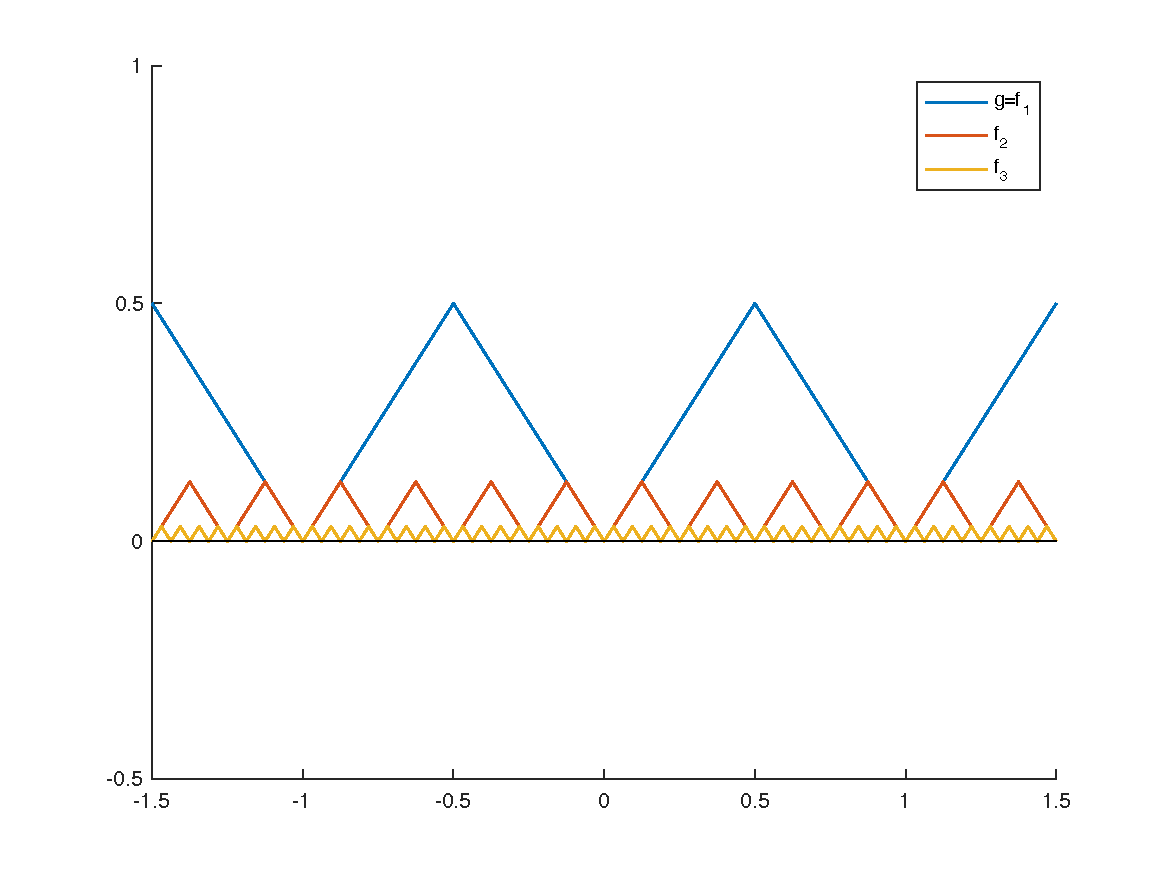
\includegraphics[scale=0.5]{fig/f3.pdf}
		\end{figure}

	\item In order to apply the Weierstrass-$M$ test, we need to find $M_n$ such that
		\begin{enumerate}
			\item $|f_n(x)| \leq M_n$ for all $x \in \mathbb{R}$ and
			\item $\sum_{n=1}^{\infty} M_n$ converges.
		\end{enumerate}
		Since $0 \leq g(x) \leq 1/2$ for all $x$, we can derive the bound
		\[
			|f_n(x)| = \left| \frac{g(4^{n-1}x)}{4^{n-1}}  \right| \leq \frac{1}{2 \cdot 4^{n-1}} \leq \frac{1}{4^{n-1}} .
		\] Then we if let $M_n = \frac{1}{4^{n-1}} $, condition (a) is satisfied. Now the infinite series $\sum_{n=1}^{\infty} M_n$ evalutes to
		\[
			\sum_{n=1}^{\infty} M_n = \sum_{n=1}^{\infty} \frac{1}{4^{n-1}} = \sum_{n=0}^{\infty} \left( \frac{1}{4} \right)^n,
		\] which converges since it is a geometric series with $|r| = 1/4 < 1$. Thus by the Weierstrass-$M$ test, $\sum_{n=1}^{\infty} f_n$ converges uniformly to $f$. Since each $f_n$ is continuous, this means $f$ is also continuous.

	\item Fix $x$, then we can find an integer $k$ such that
		 \[
			 \frac{k}{4^{m-1}} \leq x \leq \frac{k+1}{4^{m-1}} .
		 \] Denote the left fraction by $\alpha_{m-1}$ and the right fraction by $\beta_{m-1}$, then we have $\beta_{m-1}-\alpha_{m-1}=1/4^m$. Since this approaches 0 as $m$ increases and since $x$ is sandwiched between the sequence of $\alpha_m$ and $\beta_m$, the derivative of $f$ at $x$ can be written
		 \begin{align*}
			 f'(x) &= \lim_{m \to \infty} \frac{f(\beta_{m-1}) - f(\alpha_{m-1})}{\beta_{m-1}-\alpha_{m-1}} \\
			       &= \lim_{m \to \infty} \frac{\sum_{n=1}^{\infty} \left( 1/4 \right)^{n-1} \left[ g(4^{n-1} \frac{k+1}{4^{m-1}}) - g(4^{n-1} \frac{k}{4^{m-1}} ) \right]}{\beta_{m-1} - \alpha_{m-1}} \\
			       &= \lim_{m \to \infty} \frac{\sum_{n=1}^{\infty} (1/4)^{n-1} \left[ g(4^{n-m} (k+1)) - g(4^{n-m} k) \right]}{\beta_{m-1} - \alpha_{m-1}}.
		 \end{align*} In order to simplify this rather unwieldy expression, we consider how the term $G_{n,m} \doteq g(4^{n-m} (k+1)) - g(4^{n-m} k)$ changes for different values of $n$ and $m$.

		 When $n \geq m$, $4^{n-m} (k+1)$ and $4^{n-m} k$ are both integers, i.e. they are roots of $g$, so $G_{n,m}=0$. When $n < m$, $4^{n-m} (k+1)$ and $4^{n-m} k$ lie within consecutive integers, so their difference is just $G_{n,m}= 4^{n-m}$.

		 Thus we can rewrite our expression for the derivative as
		 \begin{align*}
			 f'(x) &= \lim_{m \to \infty} \frac{\sum_{n=1}^{m}(1/4)^{n-1} 4^{n-m} + \sum_{n=m+1}^{\infty} 0}{\beta_{m-1} - \alpha_{m-1}} \\
			       &= \lim_{m \to \infty} \frac{ \sum_{n=1}^{m} 4^{-m+1}}{1/4^m} \\
			       &= \lim_{m \to \infty} \frac{4^{-m+1}m}{1/4^m} \\
			       &= \lim_{m \to \infty} 4m.
		 \end{align*}
		 This clearly diverges, so $f$ cannot be differentiable at $x$. Since $x$ was arbitrary, this shows that $f$ is nowhere differentiable.

\end{enumerate}

\end{document}
